\newcommand{\mcG}{\mathcal{G}}
\newcommand{\mcV}{\mathcal{V}}
\newcommand{\mcE}{\mathcal{E}}
\newcommand{\bfitx}{\symbfit{x}}
\newcommand{\Wq}{\symbfit{W}_q}
\newcommand{\Wk}{\symbfit{W}_k}
\newcommand{\Wv}{\symbfit{W}_v}

\newcommand*{\ldblbrace}{\{\mskip-4mu\{}
\newcommand*{\rdblbrace}{\}\mskip-3mu\}}

\chapter{Basics of Geometric Deep Learning and Graph Neural Networks}\label{chap:gnn}

\section{Graphs}\label{sec:graphs}

In various branches of science, from biology to particle physics, graphs are often used as models of systems of relations and interactions. In this work, graphs are important as they engender a fundamental type of permutation invariance.

A basic \textbf{graph} \(\mcG=\left(\mcV, \mcE \right)\) is a collection of \textbf{nodes} $\mcV$ and \textbf{edges} \(\mcE\subseteq \mcV \times \mcV\) between pairs of nodes. Depending on the application or field, the nodes can also be called \textbf{vertices}, and the edges can be called \textbf{links} or \textbf{relations}.

For the purpose of an intuitive explanation, we assume that the nodes are associated with $s$-dimensional \textit{node features}, denoted by $\symbfit{x}_u$ for all $u \in \mcV$. Social networks are one of the most studied and best examples of graphs in the real world. Here, nodes represent users, edges correspond to friendship relations between them, and node features ($\symbfit{x}_u \in \mathbb{R}^d$) model user information such as age, location, last active time, etc. It should be noted that it is often possible to equip edges with features.
%however, this is not of concern within the scope of this work. Please refer to the detailed geometric deep learning text by \textcite{Bronstein2021}.


\begin{wrapfigure}{r}{0.25\textwidth}
    \centering
    % \captionsetup{justification=RaggedRight}
    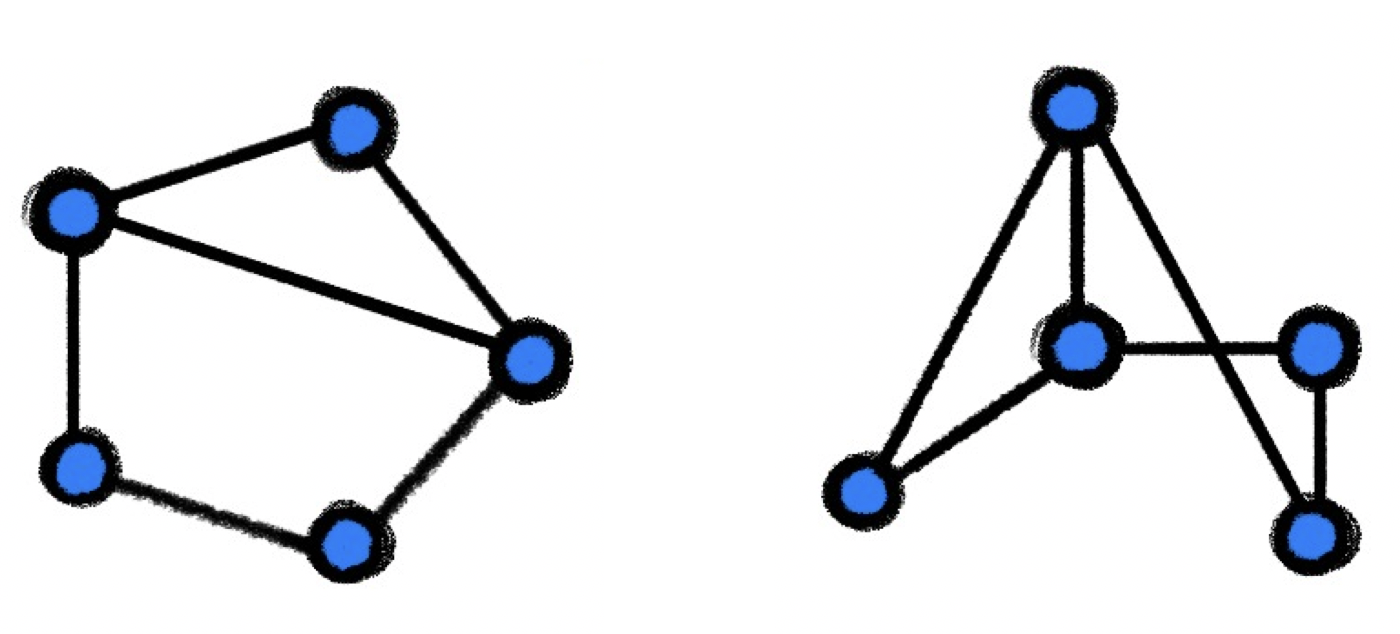
\includegraphics[scale=0.15]{chapters/assets/graph-figs/mn_isomorphic.png}
    \caption{Two isomorphic graphs.}
    \label{fig:graph-isomorphism}
\end{wrapfigure}
A key property of graphs is that nodes in $\mcV$ are not typically assumed to be provided in any particular ordering, and thus, by extension, any operations performed on graph structures should not depend on any assumed inherent ordering of nodes. The desirable property that functions acting on graphs must possess is called \textbf{permutation invariance}, and implies that for any two \textbf{isomorphic} graphs, the results of such functions must be identical. {\em Isomorphism} is an edge-preserving bijection between two graphs. The two isomorphic graphs shown in \cref{fig:graph-isomorphism} are identical up to the reordering of their nodes.

Permutation invariance is important in \samptr{}(see \Cref{chap:samp-transfer-art}). One of the main motivations behind \samptr\ is to allow the network to learn from multiple samples made available to the network in the form of a mini-batch. The ordering of the samples is of little interest to us, as we are more concerned with learning by looking beyond single instances. The exact mechanism of this will be explained in more detail in subsequent sections.


\section{Janossy Pooling}\label{sec:janossy-pooling}
Let us first illustrate the concept of permutation invariance on \textbf{sets}, a special case of graphs without edges ($\mcE=\emptyset$). We illustrate this with the help of a framework provided to us in the form of Janossy pooling \parencite{Murphy2018}.

Currently, there are a few ways to incorporate permutation invariance. The first is the ``permute and average'' paradigm. It works by considering all possible permutations of input elements, then passing each permutation through a permutation-sensitive model or function, and then taking an average of all the results. If two inputs $\symbfit{X}$ and $\Tilde{\symbfit{X}}$ are permutations of each other, this process will give the same result for both inputs. Mathematically, this can be written as follows:
\begin{equation}
    \label{eqn:perm-invar-avg}
    \widehat{f}(\symbf{X}) = \frac{1}{|{T}_n|} \sum_{\pi \in {T}_n} \phi \bigl( \pi \left( \symbf{X} \right) \bigr)
\end{equation}
where $\symbfit{X}=\left[\symbfit{x}_1^\top, \ldots, \symbfit{x}_n^\top\right]^\top$ is a stack of node features and has $n$ elements with $d$ dimensionality, $T_n$ is the set of all permutations of $n$ elements, and $\phi$ is a permutation-sensitive model. Therefore, we construct a permutation-invariant $\widehat{f}$ from a permutation-sensitive $\phi$.

This idea is called \textbf{Janossy pooling} and was first introduced by \textcite{Murphy2018}. Indeed, it is a straightforward and easy way to achieve permutation invariance, but it happens to be very computationally intensive. The computational cost is dominated by the sum over $T_n$ in \cref{eqn:perm-invar-avg}, where the number of elements in $T_n$ is $n!$. As one can imagine, if $\symbfit{X}$ is a mini-batch with very large $n$, \cref{eqn:perm-invar-avg} quickly becomes intractable.

\begin{figure}[bh]
    \centering
    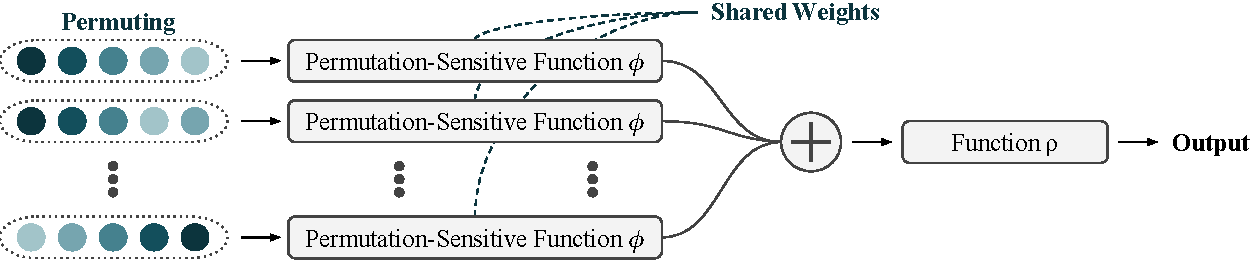
\includegraphics[width=\textwidth]{chapters/assets/graph-figs/permuting.pdf}
    \caption{$\widehat{f}$ comprises everything up to and including the sum. The function $\rho$ applied after the sum is optional and does not need to follow any constraints to guarantee invariance because its input, $\widehat{f}(x)$, is already invariant. Image courtesy of \textcite{wagstaff2022universal}.}
    \label{fig:basic-perm-invar}
\end{figure}
% \footnotetext{\url{https://fabianfuchsml.github.io/learningonsets}}

\subsection{A More Efficient Janossy Pooling}\label{ssec:efficient-janossy}

To save computational costs, we may give up the calculation of $n!$ permutations. In the above \Cref{fig:basic-perm-invar}, we look at all possible $n$-tuples from the set of $n$ elements; instead, we can consider all $k$-tuples where $k \less n$ \parencite{Murphy2018}. We can then update \cref{eqn:perm-invar-avg} as:
\begin{equation}
    \label{eqn:k-tup-janossy}
    \widehat{f}(\symbfit{X}) = \frac{1}{|P(n, k)|} \sum_{\symbfit{X}_{\{k\}}} f(\symbfit{X}_{\{k\}})
\end{equation}
where $\symbfit{X}_{\{k\}}$ stands for a $k$-tuple of $\symbfit{X}$.

Let us take a short example to understand how the count of values came about in \cref{eqn:k-tup-janossy}. Consider the input set ${w, x, y, z}$ with $n=4$. When we set $k=2$, then our sum will be applied over all $2$-tuples:
\[(w, x),~(x, w),(w, y),~(y, w),~(w, z),~(z, w),
(x, y),~(y, x),~(x, z),~(z, x),~(y, z),~(z, y)
\]
A sum over all these tuples is clearly invariant to permutations of elements in the input set, that is, each tuple appears exactly once in the sum no matter the order of individual elements. Therefore, the number of $k$-tuples from a set of $n$ elements is:
\begin{equation}
\label{eqn:k-tup-cnt}
    P(n,k) = \frac{n!}{(n-k)!}
\end{equation}

For $k \ll n$, this gives us a much more tractable method. Setting $k=n$ gives us the most expressive and most expensive model. Setting $k=1$ gives us a model whose cost is linear in the size of the input set. Increasing $k$ allows us to take into account higher-order interactions between elements in the set; we will come back to this idea of interactions in \Cref{ssec:relation-and-interactions}.

\begin{figure}[th]
    % \vspace{-0.2cm}
	\centering
% 	\hspace{-1cm}
	\begin{subfigure}[h]{0.46\textwidth}
		\centering
		\captionsetup{justification=centering}
		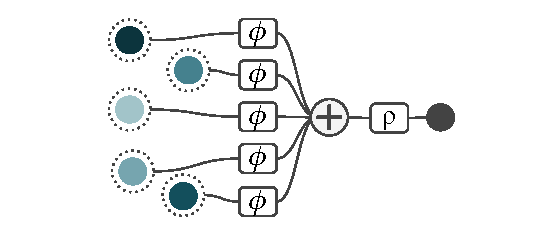
\includegraphics[width=0.99\textwidth]{chapters/assets/graph-figs/Janossy_K1.pdf}
		\caption{Janossy pooling with $k=1$ (\emph{Deep Sets})}
		\label{fig:Janossy_K1}
	\end{subfigure} 
	\begin{subfigure}[h]{0.46\textwidth}
		\centering
		\captionsetup{justification=centering}
		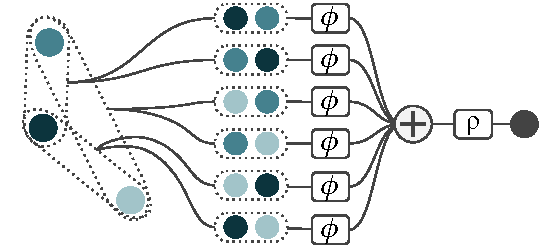
\includegraphics[width=0.99\textwidth]{chapters/assets/graph-figs/Janossy_K2.pdf}
		\caption{Janossy pooling with $k=2$}
		\label{fig:Janossy_K2}
	\end{subfigure} 
	\begin{subfigure}[h]{0.46\textwidth}
	    \vspace{+1cm}
		\centering
		\captionsetup{justification=centering}
		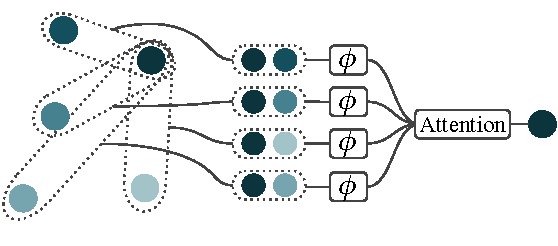
\includegraphics[width=0.99\textwidth]{chapters/assets/graph-figs/Janossy_K2Att.pdf}
		\vspace{-0.8cm}
		\caption{Self-attention}
		\label{fig:Janossy_K2Att}
	\end{subfigure} 
	\caption{Different variations of Janossy pooling. Permutation invariance is guaranteed by processing all combinations of $k$ elements and then aggregating via a sum (or softmax in the case of attention). Self-attention, a variant of Janossy pooling with $k=2$, focuses on one node at a time (the darkest node here), computing an output for this specific node. It is often employed for all nodes in parallel in a permutation-equivariant manner, mapping sets of points to sets of points \parencite{Lee2018}. Image borrowed from \textcite{wagstaff2022universal}.}
	\label{fig:k12}
\end{figure}

\subsection{Deep Sets}\label{ssec:deep-sets}

When $k=1$ and we include the optional function $\rho$, we obtain a popular special case known as Deep Sets \parencite{zaheer2017deep}. \citeauthor{zaheer2017deep} propose a neural architecture in which each input is first transformed by a neural network model $\phi$ individually (see \Cref{fig:Janossy_K1}), then the results are aggregated through a $\operatorname{sum}$ operator and further processed by a second neural network $\rho$.

The aforementioned functions produce a \textquote{global} graph-wise result, but we are frequently more interested in functions that work \textquote{locally} or node-wise. In order to acquire the collection of latent node features, for instance, we would wish to use some function to \textit{update} the features in each node. In other words, we may wish for a \textbf{node-wise} function to be permutation equivariant and want a permutation invariant \textbf{graph-wise} function.

We can now generalise the notions of permutation-invariance and equivariance from sets to graphs. In the generic setting $\mcE \neq \emptyset$, the graph connectivity can be represented by a $n \times n$ \textbf{adjacency matrix} $\symbfit{A}$, defined as
\begin{equation}
    \label{eqn:adj-matrix-def}
    a_{u v}= \begin{cases}1 & (u, v) \in \mcE \\ 0 & \text { otherwise }.\end{cases}
\end{equation}

Note that now the adjacency and input (or feature) matrices $\symbfit{A}$ and $\symbfit{X}$ are \textquote{synchronised}, $a_{u, v}$
specifies the adjacency information between the nodes described by the $u\textsuperscript{th}$ and $v\textsuperscript{th}$
rows of $\symbfit{X}$. Therefore, applying a permutation matrix $\symbfit{P}$ to node features $\symbfit{X}$ directly implies applying it to $\symbfit{A}$'s rows and columns, $\symbfit{PAP}^\top$. We then say that a graph-wise function $f$ is permutation invariant if 
\begin{equation}
    f\left(\symbfit{P X}, \symbfit{P A}^{\top}\right)=f(\symbfit{X}, \symbfit{A})
\end{equation}
and a node-wise function $\rho$ is permutation equivariant if
\begin{equation}
    \rho\left(\symbfit{P X}, \symbfit{P A P}^{\top}\right)=\symbfit{P}\rho(\symbfit{X}, \symbfit{A})
\end{equation}

\subsection{Modelling Relations and Interactions}\label{ssec:relation-and-interactions}

\samptr{} has yet another fundamental idea that is essential for its success and operation. 
It is able to exploit the interactions (or relations) between elements in a mini-batch, which really means that we are trying to capture the fact that our model output may depend not only on the individual contribution of each element, but it may be crucial to also take into account the fact that certain elements appear together in the same set. Our goal is simply to model and use these interactions.

To illustrate this with a simple example, imagine the task of evaluating how well a set of ingredients work together to cook a meal. Setting $k=1$ allows the function $\phi$ to consider related individual attributes, but cannot detect conflicts between ingredients (e.g., garlic vs. caramel). A larger $k$ allows $\phi$ to see more than one item at a time, allowing it to make relational inferences about pairs of ingredients, allowing for a more expressive model of deliciousness. Considering $\phi$ as an encoder and $\rho$ as a decoder, $\phi$ can encode information about interactions, which $\rho$ can use for decoding.

Similar to the above example, $\samptr$ uses contrastive learning (see \Cref{sec:contrastive-learning}) in order to learn to place semantically similar images closer together in an embedding space. When we increase $k$, we give our model the expressivity to learn to recognise semantic similarities between images and to explicitly take these relations into account. By allowing the model to consider relations between images in a mini-batch, it can better decide which images belong closer together in the feature space and in turn learn better discriminative semantic features. Bear in mind that the image is first passed through a CNN (see \Cref{chap:cnn}), and all the other operations explained here are applied to the flattened output of the CNN.


\section{Janossy Pooling and Self-Attention}\label{sec:jan-attn}

Many of the current neural architectures resemble Janossy pooling with $k=2$.
\textbf{Self-attention} \parencite{vaswani2017attention} is one such algorithm that is also used in the context of graphs in \samptr. Self-attention works by comparing two elements of a set at a time, usually by performing a scalar product.
The results of the scalar products are used as \textbf{attention weights} to aggregate information from different points using a weighted permutation invariant sum. Although it is similar to binary ($k=2$) Janossy pooling, self-attention also uses $\operatorname{softmax}$ to ensure that the attention weights sum up to $1$ (see \Cref{sec:softmax}).

To substantiate the relationship between permutation-invariant binary Janossy pooling and self-attention, we first define a natural extension of $k$-ary Janossy pooling from permutation \textit{invariance to equivariance}. In normal binary Janossy pooling, the function $\phi$ acts on every two-tuple, followed by the $\operatorname{sum}$-pooling operation. For the purpose of visualisation and intuition, we will write these two-tuples as a matrix:
\begin{equation}
    \begin{bmatrix}
    \phi(\bfitx_1, \bfitx_1) & \phi(\bfitx_2, \bfitx_1) & \cdots & \phi(\bfitx_n, \bfitx_1) \\
    \phi(\bfitx_1, \bfitx_2) & \phi(\bfitx_2, \bfitx_2) & \cdots & \phi(\bfitx_n, \bfitx_2) \\
    \vdots                   &  \vdots              & \ddots & \vdots         \\
    \phi(\bfitx_1, \bfitx_n) & \phi(\bfitx_2, \bfitx_n) & \cdots & \phi(\bfitx_n, \bfitx_n)
    \end{bmatrix}
    \label{eqn:jan-attn-matrix}
\end{equation}

If we pool over the \textit{entire matrix} we get an invariant output. However, by pooling over \textit{each row individually} we get a permutation equivariant output.
In general, we define $k$-ary equivariant Janossy pooling as follows: the $i\textsuperscript{th}$ output is obtained by aggregating the overall ($\phi$-transformed) $k$-tuples which start with the element $\bfitx_i$. A second network $\rho$ may then further transform each output individually. Mathematically, this reads as follows:
\begin{equation}
    \symbfit{z}_i = f_i(\symbfit{x}) = \rho \left( \sum_j \phi(\bfitx_i, \bfitx_j) \right).
    \label{eqn:janossy-attention}
\end{equation}

In practise, however, the process is slightly more involved. Typically, $\phi(\bfitx_i, \bfitx_j)$ is divided into \textbf{attention weights} $a(\bfitx_i, \bfitx_j)$ and \textbf{values} $v(\bfitx_j)$ and a softmax is applied on the attention weights. Furthermore, the attention weights themselves would be born from the scaled dot-product between two affine transformations called the \textbf{query} and \textbf{key}.
However, the elegant view from the lens of binary Janossy pooling remains clear. We shall come back to self-attention and its usage in $\samptr$ in later sections.

\subsection{Query, Key and Value}\label{sec:attn-qkv}
We have already alluded to queries, keys, and values in \Cref{eqn:janossy-attention}, these three entities form the major components of self-attention. These entities are also what makes self-attention based GNNs more expressive than the standard attention scheme (\Cref{eqn:attn-gnn}) \parencite{brody2021attentive, Bronstein2021, Dwivedi2020}.

Every graph attention layer uses each input node $\bfitx_i$ in three different ways:
\begin{itemize}
    \item It is compared to every other vector to establish the weights for its own output $\symbfit{z}_i$
    \item It is compared to every other vector to establish the weights for the output of the $j\textsuperscript{th}$ vector $\symbfit{z}_j$
    \item It is used as part of the weighted sum to compute each output vector once the weights have been established.
\end{itemize}

These roles are called \textbf{query}, \textbf{key}, and \textbf{value}, respectively. Each input node $\bfitx_i$ is linearly transformed three different times to derive a new vector for each of the roles. In other words, we use three $d\times d$ weight matrices $\Wq$, $\Wk$ and $\Wv$ to compute three linear transformations:
\begin{equation}
    \symbfit{q}_{i}=\symbfit{W}_{q} \bfitx_{i} \quad \symbfit{k}_{i}=\symbfit{W}_{k} \bfitx_{i} \quad \symbfit{v}_{i}=\symbfit{W}_{v} \bfitx_{i}
\end{equation}
these transformations allow the attention module a fair degree of flexibility, allowing it to project the input to suit the roles they must be a part of. 

The softmax function can be sensitive to very large input values. These kill the gradient, slow down learning, or cause it to stop altogether. Since the average value of the dot product increases with embedding dimension $d$, it helps to scale the dot product back a little to prevent the inputs to the softmax function from growing too large.
\begin{equation}
\label{eqn:qkv-attn-weight-calc}
\begin{split}
    a^\prime_{i, j} &= \frac{\symbfit{q}_i^\top \symbfit{k}_j}{\sqrt{d}}\\
    % a_{i j}& =\frac{\exp a_{i j}^{\prime}}{\sum_{j} \exp a_{i j}^{\prime}}
    a_{i, j} &= \operatorname{softmax}\left( a^\prime_{i, j} \right)\\
\end{split}
\end{equation}

\begin{tcolorbox}[title=Why $\sqrt{d}$?]
Consider a vector in $\mathbb{R}^d$ with all values $c$. Its Euclidean length is $\sqrt{d}c$. Therefore, we are dividing out the amount by which the increase in dimension increases the length of the average vectors.
\end{tcolorbox}

We then use the attention weights calculated in \Cref{eqn:qkv-attn-weight-calc}, to compute a weight sum to generate the output vector. Note that the output vector $\symbfit{z}_i$ depends on $\symbfit{v}_j, \forall j$ however not every $\symbfit{v}_j$ contributes equally to output $\symbfit{z}_i$. The contribution to the output is controlled by the attention weight $a_{i, j}$:
\begin{equation}
    \label{eqn:qkv-attn-aggregation}
    \symbfit{z}_{i}=\sum_{j} a_{i, j} \symbfit{v}_{j}.
\end{equation}

As stated in \Cref{sec:janossy-pooling,sec:graph-nn}, self-attention is a special case of graph neural networks and was first proposed by \textcite{vaswani2017attention}. We can see this from \Cref{eqn:qkv-attn-aggregation,eqn:janossy-attention}. We can also view this from the message-passing perspective presented in \Cref{sec:graph-nn} to realise that every output is determined by all its neighbours; it is this structure that $\samptr$ successfully makes use of in order to \textquote{look} beyond single instances and refine features.

\newpage
\section{Graph Neural Networks}\label{sec:graph-nn}

Now that we have described graphs and permutation invariant and equivariant functions, we can begin to talk about Graph Neural Networks (GNNs). GNNs are perhaps among the most \textbf{general} class of deep learning architectures in existence at this moment. Some deep learning architectures can be understood as special cases of the GNN with additional geometric structure. As it happens, we have already covered one such specific case, self-attention in \cref{sec:jan-attn}.

Notice that in \Cref{sec:jan-attn}, the output of $i\textsuperscript{th}$ depends on all pairs of $(i, j)$. However, we can also constrain this so that the $i\textsuperscript{th}$ output is more dependent on \textbf{local} nodes. This means that instead of considering all pairs, the output of node $i$ instead depends on a smaller set of neighbours. We can formalise this to define what we mean when a node is a  \textquote{neighbour} of another node.

The \textbf{neighbourhood} of $i$ is defined as:
\begin{equation}
\mathcal{N}_{i}=\{j:(i, j) \in \mathcal{E} \text { or }(j, i) \in \mathcal{E}\}
\end{equation}
and the neighbourhood features as the multiset:
\begin{equation}
\symbf{X}_{\mathcal{N}_{i}}=\ldblbrace\bfitx_{j}: j \in \mathcal{N}_{i}\rdblbrace .
\end{equation}

Further generalising on our perspective developed in \Cref{sec:janossy-pooling} and \Cref{sec:jan-attn}, we can specify a function $\varphi(\bfitx_i, \symbf{X}_{\mathcal{N}_{i}})$ that is locality aware and can operate over a node and its neighbourhood. Then a permutation equivariant function $h$ can be constructed by applying $\varphi$ to every node's neighbourhood separately:
\begin{equation}
    h({\symbf X}, {\symbfit A}) =
\left[
  \begin{array}{ccc}
     & \varphi(\bfitx_1, \symbf{X}_{\mathcal{N}_1}) &  \\
     & \varphi(\bfitx_2, \symbf{X}_{\mathcal{N}_2}) &  \\
             & \vdots    &          \\
     & \varphi(\bfitx_n, \symbf{X}_{\mathcal{N}_n}) & 
  \end{array}
\right].
\label{eq:graph_equivariant}
\end{equation}

As $h$ is constructed by applying a shared function $\varphi$ to each node locally, its permutation equivariance rests on the output of $\varphi$ being independent of the ordering of the nodes in $\mathcal{N}_i$. Therefore, if $\varphi$ is built to be permutation invariant, then this property will be satisfied. Observe that the role $\varphi$ plays here is that of $\widehat{f}$ in \Cref{eqn:perm-invar-avg} and role played by $h$ is similar to that of $f$ in \Cref{eqn:janossy-attention}.

\begin{figure}[th]
    \centering
    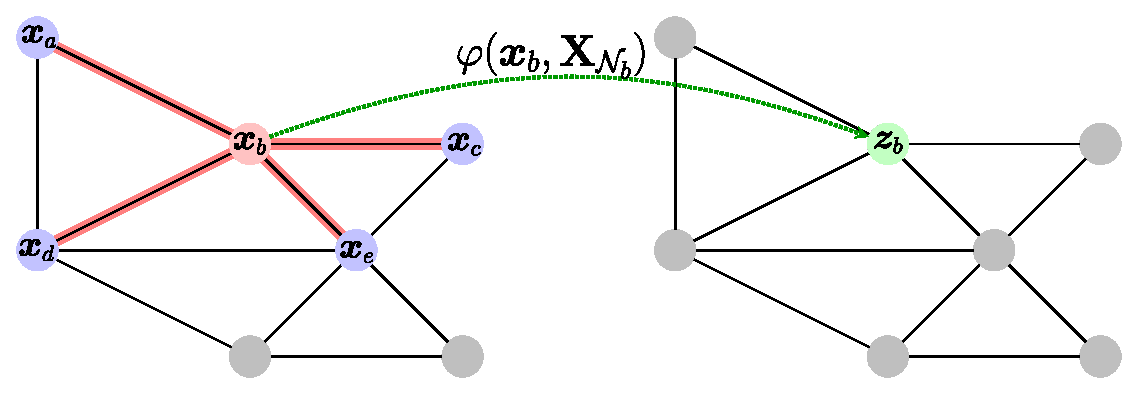
\includegraphics[width=\linewidth]{chapters/assets/graph-figs/GC_GDL.eps}
    \caption{By applying a permutation-invariant function $\varphi$ to every neighbourhood. In this case, $\varphi$ is applied to the features $\bfitx_b$ of node $b$ as well as the multiset  of its neighbourhood features, $\symbf{X}_{\mathcal{N}_b} = \ldblbrace\bfitx_a, \bfitx_b, \bfitx_c, \bfitx_d, \bfitx_e\rdblbrace$. Applying $\varphi$ in this manner to every node's neighbourhood recovers the rows of the resulting matrix of latent features $\symbf{Z}=h(\symbf{X}, \symbfit{A})$. Image modified from \parencite{Bronstein2021}.}
    \label{fig:gc_gdl}
\end{figure}%

A GNN is a optimisable transformation on the attributes of a graph (nodes, edges, global context) that preserves permutation invariance.
Based on our discussion in \Cref{ssec:deep-sets}, we consider a graph to be specified with an adjacency matrix $\symbfit{A}$ and node features $\symbf{X}$. We will discuss GNN architectures that are \textbf{permutation equivariant} functions $h(\symbf{X}, \symbfit{A})$ constructed by applying shared permutation invariant functions $\varphi(\bfitx_i, \symbf{X}_{\mathcal{N}_i})$ where $\symbf{X}_{\mathcal{N}_i}$ is the neighbourhood of $\bfitx_i$. This local function $\varphi$ can be referred to as \textquote{diffusion}, \textquote{propagation}, or \textquote{message-passing}, and the computation $h$ is referred to as a GNN layer.

\begin{figure}
    \centering
    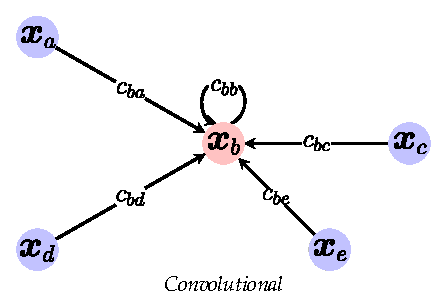
\includegraphics[width=0.33\linewidth]{chapters/assets/graph-figs/GNN_GDL_TYPES_C.eps}
    \hspace{-0.5em}
    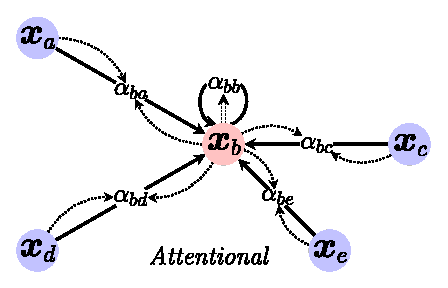
\includegraphics[width=0.33\linewidth]{chapters/assets/graph-figs/GNN_GDL_TYPES_A.eps}
    \hspace{-0.5em}
    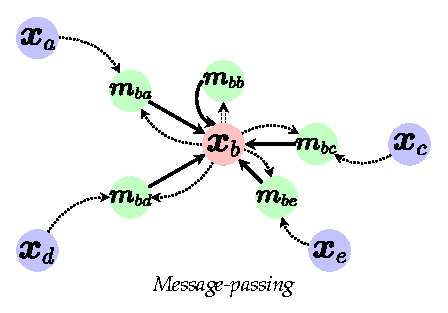
\includegraphics[width=0.33\linewidth]{chapters/assets/graph-figs/GNN_GDL_TYPES_MP.eps}
    \caption{A visualisation of the dataflow for the three flavours of GNN layers, $g$. We use the neighbourhood of node $b$ from Figure \ref{fig:gc_gdl} to illustrate this. Left-to-right: \textbf{convolutional}, where sender node features are multiplied with a constant, $c_{uv}$; \textbf{attentional}, where this multiplier is \emph{implicitly} computed via an attention mechanism of the receiver over the sender: $\alpha_{ij}=a(\vec{x}_i, \vec{x}_j)$; and \textbf{message-passing}, where vector-based messages are computed based on both the sender and receiver: $\vec{m}_{ij}=\psi(\vec{x}_i, \vec{x}_j)$. Image modified from \parencite{Bronstein2021}.}
    \label{fig:gc_flavours}
\end{figure}%

There are three types of GNN layers that are most common, in all three of them permutation invariance is satisfied by \textbf{aggregating} features from $\symbf{X}_{\mathcal{N}_i}$ (potentially transformed by another function $\psi$) with some permutation-invariant function $\bigoplus$, and then \textbf{updating} the features of node $i$, by means of some function $\varphi$. Usually, $\varphi$ and $\psi$ are learnable affine transformations with activation functions (see \Cref{chap:basics-of-dl}) and $\bigoplus$ is an operation such as $\operatorname{sum}$, $\operatorname{mean}$, or $\operatorname{max}$. These operations are analogous to pooling functions discussed in \Cref{sec:conv-pooling}.

In the \textbf{convolutional} kind of GNNs \parencite{kipf2016semi}, the features of the neighbourhood nodes are directly aggregated with fixed weights,
\begin{equation}
    z_{u}=\varphi\left(\bfitx_{i}, \bigoplus_{j \in \mathcal{N}_{i}} c_{i j} \psi\left(\bfitx_{j}\right)\right).
    \label{eqn:gcn}
\end{equation}
Here, $c_{ij}$ specifies the importance of node $i$ to node $j$'s representation.

In the \textbf{attentional} scheme \parencite{velic018graph, brody2021attentive}, the interactions are implicit.
\begin{equation}
z_{i}=\varphi\left(\bfitx_{u}, \bigoplus_{j \in \mathcal{N}_{i}} a\left(\bfitx_{i}, \bfitx_{j}\right) \psi\left(\bfitx_{j}\right)\right)
\label{eqn:attn-gnn}
\end{equation}
Here, $a$ is a learnable \textbf{self-attention} mechanism that computes the importance coefficients $\alpha_{ij} = a(\bfitx_i,\bfitx_j)$ implicitly. They are often softmax-normalised across all neighbours. If the aggregation operation $\bigoplus$ is summation, then the aggregation is a linear combination of the neighbourhood node features, but the weights are feature-dependent. The reader is urged to recognise the similarities between \Cref{eqn:attn-gnn} and \Cref{eqn:janossy-attention}.

Finally, the \textbf{message-passing} type amounts to computing arbitrary vectors (\textquote{messages}) across edges,
\begin{equation}
    z_{i}=\varphi\left(\bfitx_{i}, \bigoplus_{j \in \mathcal{N}_{i}} \psi\left(\bfitx_{i}, \bfitx_{j}\right)\right)
    \label{eqn:mesg-passing}
\end{equation}
Here, $\psi$ is a learnable message function, computing $j$'s vector sent to $i$, and the aggregation can be considered as a form of message passing on the graph.

It should be noted that the relationship between the three approaches is as follows \textit{convolution} $\subseteq$ \textit{attention} $\subseteq$ \textit{message-passing}. The attentional mechanism can represent convolutional GNNs by an attention-mechanism implemented as a lookup table $a(\bfitx_i, \bfitx_j) = c_{ij}$. Message-passing can represent both convolutional and attentional GNNs where the messages are only the sender node's features: $\psi(\bfitx_i, \bfitx_j)=c_{ij}\psi(\bfitx_j)$ for convolutional GNNs and $\psi(\bfitx_i, \bfitx_j)=a\left(\bfitx_{i}, \bfitx_{j}\right)\psi(\bfitx_j)$ for attentional GNNs. $\samptr$ makes use of the attentional semantics in the message-passing context to implement its GNN, however, the implementation of the attention mechanism follows \parencite{vaswani2017attention} instead of the mechanism suggested in \parencite{velic018graph}.

% \section{Self-Attention}\label{sec:self-attention}

% We shall close out the discussion on geometric deep learning and GNNs by following up on \Cref{sec:janossy-pooling} and going into a bit more detail about how self-attention is implemented. While our geometric deep learning based perspective is still valid, there are several details that affect the implementation, although the form of self-attention remains the same as we have discussed in earlier sections.

% \subsection{Query, Key and Value}\label{sec:attn-qkv}
% We have already alluded to queries, keys and values in \Cref{eqn:janossy-attention}, these three entities form the major components of self-attention. These entities are also what makes self-attention based GNNs more expressive than the standard attention scheme (\Cref{eqn:attn-gnn}) \parencite{brody2021attentive, Bronstein2021, Dwivedi2020}.

% Every graph attention layer uses each input node $\bfitx_i$ in three different ways:
% \begin{itemize}
%     \item It is compared to every other vector to establish the weights for its own output $\symbfit{z}_i$
%     \item It is compared to every other vector to establish the weights for the output of the $j\textsuperscript{th}$ vector $\symbfit{z}_j$
%     \item It is used as part of the weighted sum to compute each output vector once the weights have been established.
% \end{itemize}

% These roles are called \textbf{query}, \textbf{key}, and \textbf{value}, respectively. Each input node $\bfitx_i$ is linearly transformed three different times to derive a new vector for each of the roles. In other words, we use three $d\times d$ weight matrices $\Wq$, $\Wk$ and $\Wv$ to compute three linear transformations:
% \begin{equation}
%     \symbfit{q}_{i}=\symbfit{W}_{q} \bfitx_{i} \quad \symbfit{k}_{i}=\symbfit{W}_{k} \bfitx_{i} \quad \symbfit{v}_{i}=\symbfit{W}_{v} \bfitx_{i}
% \end{equation}
% these transformations allow the attention module a fair degree of flexibility, allowing it to project the input to suit the roles they must be a part of. 

% The \highlight[comment=write why softmax is used]{softmax} function can be sensitive to very large input values. These kill the gradient, slow down learning, or cause it to stop altogether. Since the average value of the dot product increases with embedding dimension $d$, it helps to scale the dot product back a little to prevent the inputs to the softmax function from growing too large.
% \begin{equation}
% \label{eqn:qkv-attn-weight-calc}
% \begin{split}
%     a^\prime(i, j) &= \frac{\symbfit{q}_i^\top \symbfit{k}_j}{\sqrt{d}}\\
%     % a_{i j}& =\frac{\exp a_{i j}^{\prime}}{\sum_{j} \exp a_{i j}^{\prime}}
%     a(i, j) &= \operatorname{softmax}\left( a^\prime(i, j) \right)\\
% \end{split}
% \end{equation}

% \begin{tcolorbox}[title=Why $\sqrt{d}$?]
% Consider a vector in $\mathbb{R}^d$ with values all $c$. Its Euclidean length is $\sqrt{d}c$. Therefore, we are dividing out the amount by which the increase in dimension increases the length of the average vectors.
% \end{tcolorbox}

% We then use the attention weights calculated in \Cref{eqn:qkv-attn-weight-calc}, to compute a weight sum to generate the output vector. Note that the output vector $\symbfit{z}_i$ depends on $\symbf{v}_j \forall j$ however not every $\symbfit{v}_j$ contributes equally to output $\symbfit{z}_i$. The contribution to the output is controlled by the attention weight $a(i, j)$.
% \begin{equation}
%     \label{eqn:qkv-attn-aggregation}
%     \symbfit{z}_{i}=\sum_{j} a(i, j) \symbfit{v}_{j}
% \end{equation}

% As stated earlier in \Cref{sec:janossy-pooling,sec:graph-nn}, self-attention is a special case of graph neural networks. We can see this from \Cref{eqn:qkv-attn-aggregation,eqn:attn-gnn,eqn:janossy-attention}. We can view this from the message-passing perspective presented in \Cref{sec:graph-nn} to realise that every output is determined by all its neighbours, it is this structure that $\samptr$ succesfully makes use of in order to \textquote{look} beyond single instances and refine features.